\section{Contexto conceptual}
\label{sec:conceptos}

Para comprender bien en qué consiste \fpt para alguien ajeno
a campos como la genética o la evolución biológica, hace falta antes
definir conceptos relacionados y saber exáctamente donde se enmarca el
software. Ésta sección será muy importante ya que es la que describe
la naturaleza del campo en el que está inmerso \fpt lo que nos ayuda a
comprender los problemas y las dificultades \----que se verán en las
próximas secciones\---- contra las que \fpt ha debido, debe y deberá
de enfrentarse para lograr los objetivos marcados.

\subsection{Concepto de evolución}
El concepto de evolución es a veces entendido como una vía de
progreso, desde formas inferiores o peores, a formas superiores o
mejores. En realidad, la \textbf{teoría sintética de la
  evolución}\footnote{También llamado síntesis evolutiva moderna,
  neodarwinismo o sencillamente teoría sintética.} solo se
basa en un \textbf{hecho científico}, a saber, que cualquier par
de organismos tiene un antepasado común. Ésta base tan simple no
permite otorgar ningún tipo de connotaciones de superioridad,
dominancia o dirección a la palabra \textbf{evolución}, que se define,
sencillamente, como sinónimo de \textbf{cambio}.

A grandes rasgos, la evolución funciona de la siguiente forma. Las
características de un individuo \----como la altura, fuerza física o
metabolismo\---- no son más que el reflejo de las
proteinas que existen en tu cuerpo. Como ejemplo, las células de los huesos se
distinguen de las células de la piel, en que las primeras tienen las
proteínas propias de los huesos, y las segundas tienen las proteínas
propias de la piel. Por lo demás, las células serán prácticamente
iguales. ¿Quién tiene la información de qué proteínas debes tener en
tu cuerpo?, pues el ADN, que existe en
cada una de las células de cualquier organismo. El ADN es una cadena larga de
\textbf{bases nitrogenadas}, donde solo ciertas subcadenas son las que
importan: son los llamados genes. Cada gen es un trocito de ADN que
contiene información de una proteina, y estas subcadenas corresponden,
en realidad, una minoría (salvo en bacterias), dado que la mayor parte
del ADN de una célula no sirve para nada\footnote{Ésto no es
  totalmente cierto, pero no entraré en detalles.}. Así, si cambia el ADN,
pueden cambiar tus proteinas, y si ésto ocurre \----es decir, cuando lo
que ha cambiado pertenece a un gen\----, cambian tus
características. Así que la evolución se produce porque el ADN cambia
de generación en generación, por ejemplo, mediante mutaciones (fallo
en la copia de padre a hijo), aunque existen también otros
\textbf{mecanismos de cambio}.

Pero el ADN no cambia completamente, solo cambia una pequeña
parte, y ésta parte no tiene por qué ser la misma, así que los
cambios son muy probables que se hereden a los hijos. Solo hace falta
una cosa: llegar vivo a la edad reproductiva, y además, reproducirse
\----y contra más mejor\----,
y tus nuevas características pueden cambiar la forma en que llegas a
la edad reproductiva y tu tasa de
reproducción. Éste cambio es, \textit{a grosso modo}, selección
natural en el primer caso, y lo segundo es selección sexual. Si tienes éxito
reproductivo, el porcentaje de tu gen, respecto a la población,
crecerá, o disminuirá en caso contrario. Éste porcentaje también puede
cambiar si, en vez de cambiar tus genes, cambia el medioambiente, y lo que
antes era favorable, ahora puede ser perjudicial aunque los genes no
cambien. La selección natural y sexual actuarán de igual aunque los
genes no cambien, pues solo mide como cambia tu éxito
reproductivo. Por eso a éstos mecanismos se les dice que son
mecanismos de \textit{fijación}, ya que la selección
natural\footnote{La selección sexual es, en realidad, un caso
  concreto de selección natural.} acaba por fijar el porcentaje
de ocurrencia de cada gen en la población. Por
supuesto, existen otros mecanismos de fijación además de la selección
natural.

\subsection{Concepto de clasificación}
Antes de que los científicos supieran todo ésto, la visión que se
tenía sobre la biología era muy distinta: los organismos no cambian, y
correspondían a un plan divino, a una «gran cadena del ser» (la
\textit{scala naturae}), en contraposición a la visión evolutiva, que
es un árbol fuertemente ramificado. El hombre estaba en la cima de la
escala biológica, solo por debajo de los ángeles (que ya no pertenece
al mundo biológico), y éste por debajo de Dios. En la base de la
cadena estaban los minerales. Ésta visión estaba tan arraigada que
incluso el concepto de extinción provocaba fuertes conflictos
teológicos.

Debido a que el hombre es la cima de la perfección, el que se parece
más al hombre es más perfecto. Por eso las características de los
individuos eran las que importaban. Especies que se parecen más se
clasificaban juntas. El hombre se clasificaba junto a los monos, los
grandes simios, lemures, colugos (lemures voladores) y
murciélagos, en un órden llamado primates, que significa
primeros\footnote{Los colugos y murciélagos ya no se consideran
  primates.}. Como vemos, la clasificación refleja las ideas de la
época, y antes se clasificaban conforme a las características en
común. Sin embargo, ahora se clasifican conforme a criterios
evolutivos: los que están más emparentados se clasifican juntos.

Las clasificaciones actuales se basan en \textbf{árboles
  filogenéticos}, y aquí ya nos acercamos a lo que \fpt hace. Un árbol
filogenético es un árbol que muestra las relaciones evolutivas entre
un grupo de especies. Cuando un científico quiere establecer saber la
relación evolutiva entre un grupo de especies vivas, hace un estudio
genético y establece sus relaciones, dibujando un árbol filogenético
como el de la siguiente figura, que representa la raíz del árbol
evolutivo de la vida\footnote{Es un árbol desactualizado, la filogenia
  actual de la raíz de la vida ha cambiado drásticamente en los
  últimos años}.

\begin{center}
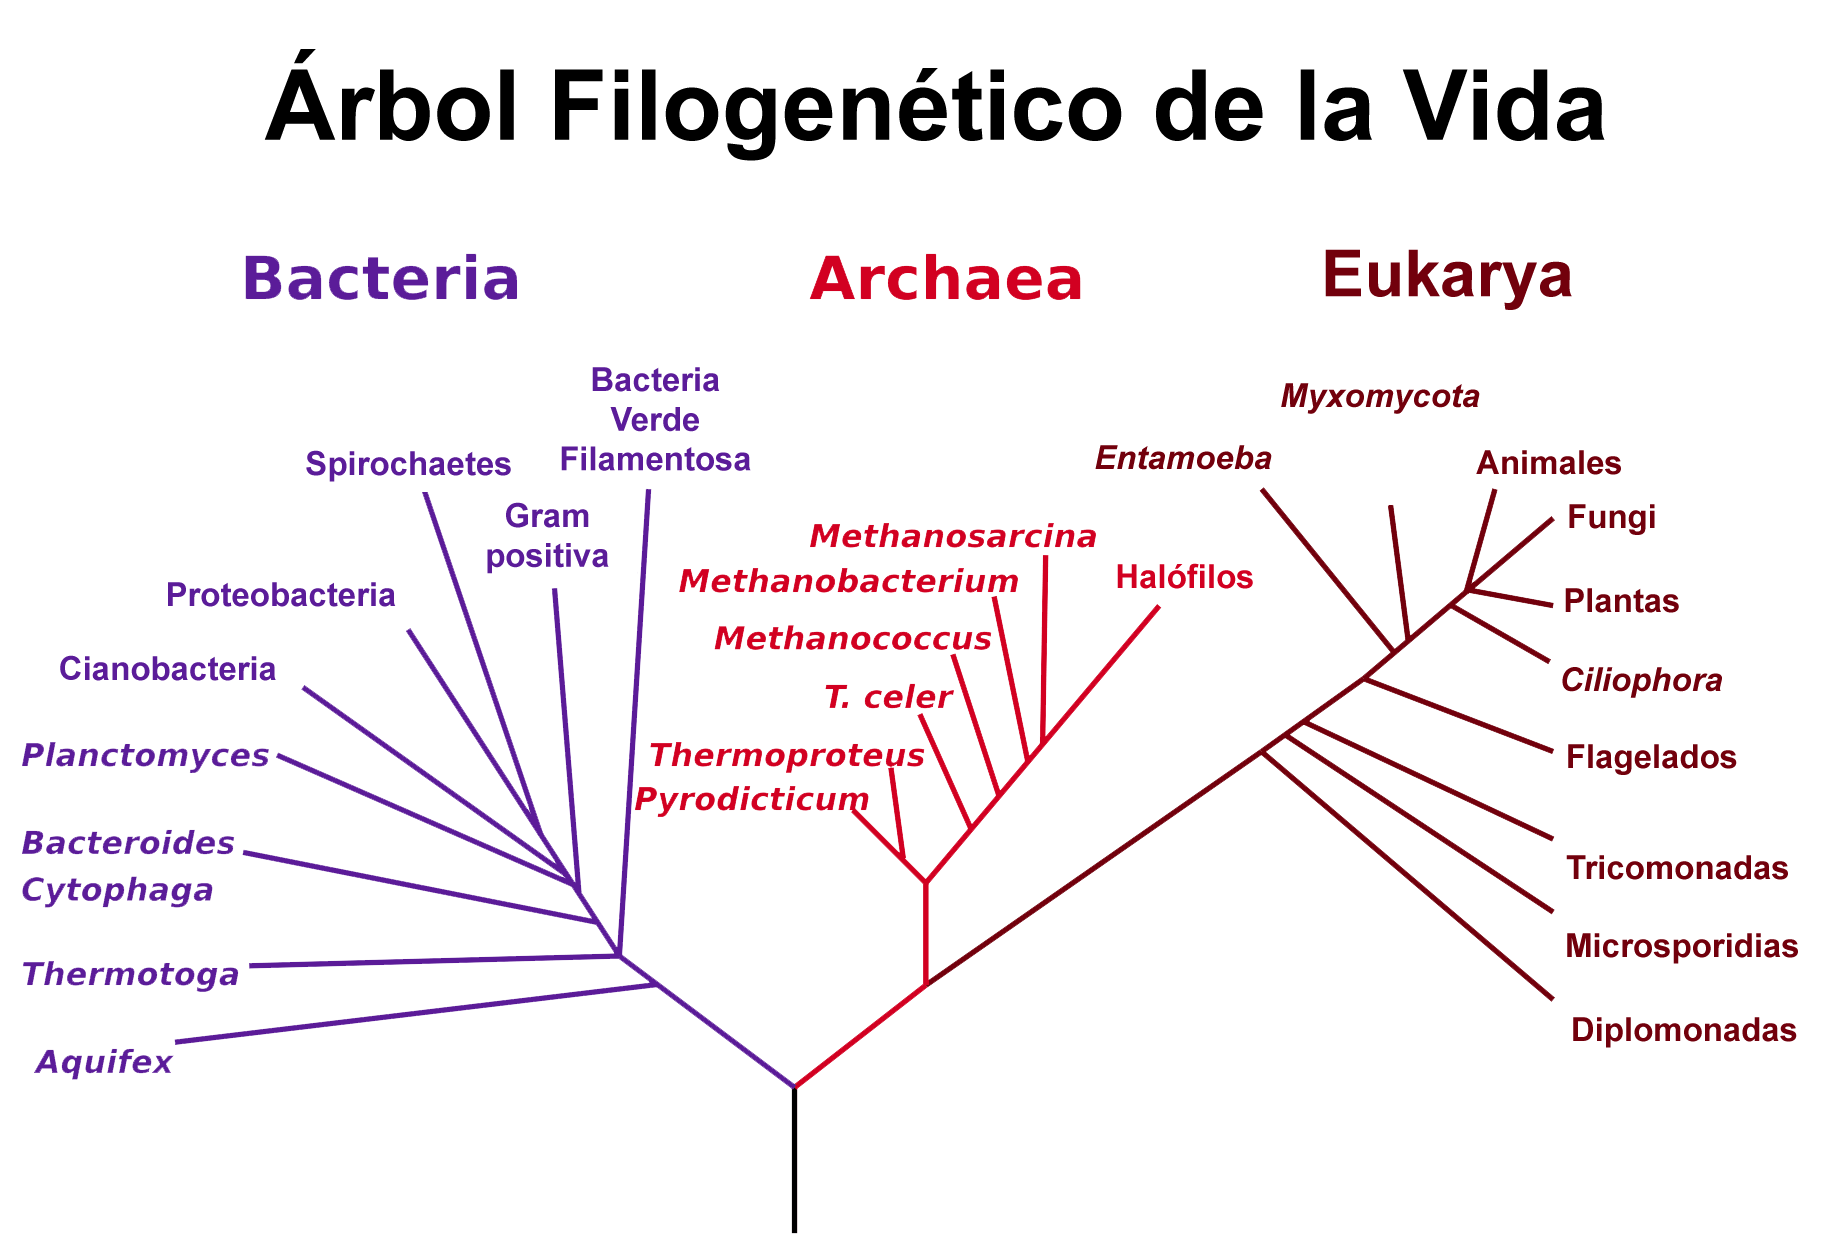
\includegraphics[scale=.2]{images/Phylogenetic_tree-es.png}
\end{center}

En estos árboles, contra más interno sea el nodo, más cercanas son las
especies que agrupa. Por ejemplo, en el árbol anterior se muestra como
los eucariontes (\textit{Eukarya}), son más cercanos a las arqueas
(\textit{Archaea}) que a las bacterias. La clasificación se realiza a
partir de éstos árboles filogenéticos: el árbol filogenético muestra
que especies están más emparentadas, y las especies más emparentadas
se clasifican juntas. Generalmente, la clasificación es una
simplificación de un árbol filogenético, ya que los árboles
filogenéticos son demasiado ramificados como para servir de
clasificación útil y cómoda.

\subsubsection{Taxonomía y sistemática}
En la ciencia de la clasificación hay que distinguir dos subciencias
que hace falta distingüir, por un lado, la \textbf{taxonomía} es la normativa
de clasificación, es decir, las reglas del juego. Ahora, se puede
jugar de muchas formas, es decir, dentro de unas mismas reglas se
puede clasificar a las especies bajo distintos enfoques. Ésto es lo
que se llama \textbf{sistemática}.

Por ejemplo, una regla dada por la taxonomía es: las especies se
clasifican usando dos nombres, el nombre del género, y el nombre de la
especie. Éstos nombres serán en latín, y se escribirán en
cursiva. El nombre del género se escribe comenzando por mayúscula, y
el nombre específico de especie únicamente en minúscula, así, en el
género \textit{homo} existen las especies \textit{Homo sapiens},
\textit{Homo   neanderthalensis}, \textit{Homo ergaster},
etcétera. También existirán, como mínimo, 6 niveles de clasificación:
reino, filo, clase, órden, familia, género y especie. Así, el hombre
pertenece al reino \textit{animalia}, al filo \textit{chordata}, clase
\textit{mammalia}, órden \textit{primates}, familia
\textit{hominidae}, género \textit{homo}, especie \textit{Homo
  sapiens}. También se pueden definir categorías intermedias para
clasificar más cómodamente a grupos muy diversos, como por ejemplo,
subfilo, superórden o infraclase. Cada elemento de la jerarquía de
clasificación se llama \textbf{taxón}. Los reglas para dar nombres a
los taxones se llama \textbf{nomenclatura biológica}.

La sistemática se encarga de definir los criterios bajo los cuales
agrupar y en qué nivel taxonómico incluyo cada grupo. Por ejemplo, las
aves evolucionan a partir de los dinosaurios, por tanto, podrías
incluir a las aves como familia del superórden \textit{dinosauria},
pero también puedes opinar que las aves son un grupo demasiado
diverso y evolucionado como para clasificarse en un nivel tan
específico, y clasificarlas en la clase \textit{aves}. Así, se definen
varias escuelas dentro de la propia sistemática, cada uno con
criterios distintos:

\begin{description}
\item[Fenética:] Clasifica a las especies según la cercanía
  morfológica, tal y como se hacía antigüamente\footnote{Los
    partidarios de la fenética moderna, evidentemente, tienen unos
    criterios totalmente distintos y científicos que los argumentos
    religiosos usados antigüamente.}.
\item[Cladística:] Todo taxón debe incluir a todos sus
  descendendientes, y así, las aves deberían incluirse \textbf{dentro}
  de \textit{dinosauria}. A cada taxón así formado se le llama un \textbf{clado}.
\item[Sistemática evolutiva:] No sólo se usan criterios evolutivos en
  la clasificación, sino también de éxito adaptativo, diversidad,
  etcétera, y así, las aves deberían incluirse en un taxón más alto de
  la jerarquía, y no dentro de \textit{dinosauria} debido a su
  condición de grupo diverso y exitoso por su adaptación a un gran
  número de nichos ecológicos distintos.
\end{description}

Como vemos, la taxonomía y la sistemática son dos ramas relativamente
desacopladas, así, la moderna clasificación basada en criterios
evolutivos se conjuga con las antigüas reglas de clasificación fijista
basada en niveles taxonómicos de filo, órden, etcétera.

Pero como pasa con todo, nada está definido de forma absoluta y sin
estar sustenta a cambios. Las escuelas cladística y la sistemática
evolutiva combaten entre sí buscando el consenso, y hay muchas
alternativas a la clasificación en cada grupo. A su vez, cada rama de
la biología tiene su propio concepto de especie, de subespecie, o
incluso la forma de clasificar; por ejemplo, en botánica, en vez de
usar el nombre de filo, se usa el nivel taxonómico de división como
sustituto. Existe el \textbf{código internacional de nomenclatura
  zoológica}, y también los correspondientes códigos internacionales
de nomenclatura en botánica, de bacterias o el \textbf{comité
  internacional de sistemática de procariotas}. También, en vez de
usar las antigüas reglas de clasificación taxonómica, la web
\textit{PhyloCode} propone una \textbf{nomenclatura filogenética} para
que las clasificaciones sean más cercanas a un árbol filogenético, y
conseguir el objetivo ideal de que cada taxón sea un clado\footnote{Un
  clado es el nombre dado a un \textbf{grupo monofilético} cuando éste
  grupo es un taxón. Un \textbf{grupo parafilético} es aquel que no
  posee a todos los descendientes, como en el caso del taxón
  \textit{dinosauria} cuando no incluye a las aves. Un \textbf{grupo
    polifilético} es aquel que contiene especies de grupos evolutivos
  distintos, como el antigüo grupo de primates, que incluía a los
  murciélagos. Actualmente, los debates se centran en si los taxones
  deberían ser grupos monofiléticos \----cladística\---- o si
  también se permiten grupos parafiléticos \----sistemática
  evolutiva\----. El consenso sí existe en el caso de los grupos
  parafiléticos, que no se permiten.}.

\subsection{Árbol filogenético}
Como hemos dicho antes, elaborar un árbol filogenético comienza
eligiendo las especies a las que se quieren conocer sus relaciones
evolutivas. Mediante estudios genéticos, puede saberse, dado un par de
\textbf{genomas} de dos individuos distintos\footnote{Genoma es el
  conjunto de genes de un individuo} la fecha en la que se produjo la
separación, es decir, la época en la que una población antecesora se
dividió en dos grupos mediante, por ejemplo, \textbf{aislamiento
  reproductivo}, ya que, a partir de ciertas tasas de cambio, el
porcentaje de diferencia representa cantidad de tiempo. A mayor
porcentaje de cambio, más antigüedad del ancestro común a
ambos. También, para estudiar las relaciones de parentesco, se acude
al estudio de las características compartidas o características
exclusivas de cada grupo; éste tipo de estudios se llaman
\textbf{análisis cladístico}.

\begin{center}
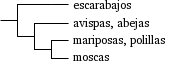
\includegraphics[scale=.7]{images/Cladogram-example1-es.png}
\end{center}

Si son tres especies las que hay que comparar, se compara por parejas
y se crea un árbol con dos escisiones, y así sucesivamente, según el
número de especies. Por eso normalmente los árboles filogenéticos son
dicotómicos, aunque también pueden haber escisiones de más elementos,
como 3 o 4, si no hay mucha diferencia temporal, aunque ésto no suele
ser muy común. A su vez, los árboles filogenéticos pueden tener muchas
apariencias. Los dos árboles filogenéticos adjuntados tienen ya una
apariencia distinta, y la siguiente imágen muestra un árbol
filogenético otra vez completamente distinto.

\begin{center}
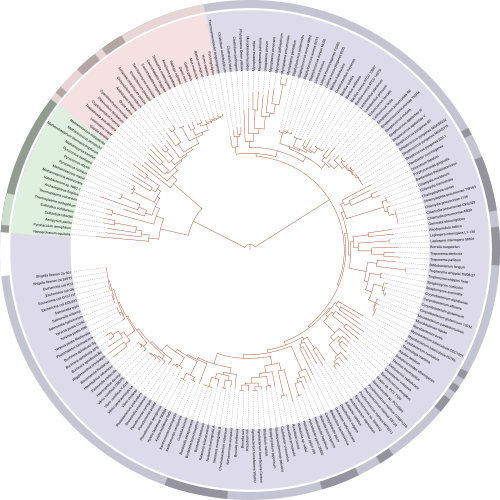
\includegraphics[scale=.7]{images/Tree_of_life.png}
\end{center}

A su vez, los árboles filogenéticos no pueden solamente variar en
forma, sino también en la información que muestra:

\begin{description}
\item[Cladograma:] Un árbol filogenético básico.
\item[Filograma:] Un árbol filogenético donde el tamaño de las aristas
  representa la cantidad de cambio.
\item[Cronograma:] Un árbol filogenético donde el tamaño de las
  aristas representa la cantidad de tiempo evolutivo.
\end{description}

El lector habrá ya advertido la raíz compartida en las palabras
cladística, clado, análisis cladístico y cladograma. El motivo de ésta
sobredominancia del término en tantos lugares distintos tiene un
motivo: el estudio filogenético es la principal vía de clasificación,y
para hacer un estudio filogenético de las especies, el
análisis cladístico es la principal vía de estudio y el resultado es
un cladograma, donde cada subárbol es un clado. Por último, la
cladística transporta éstos cladogramas a la clasificación biológica.
Además, cuando estamos tratando con fósiles y no con especies vivas,
los análisis genéticos no sirven para nada debido a que los fósiles
muy muy rara vez tienen restos de ADN, y si los tienen, éstos son
incompletos, aunque suelen servir. Por todo ésto, la cladística tiene
un papel muy importante en la sistemática biológica, y de ahí la alta
ocurrencia del término en éste documento.
